\chapter{HASIL DAN PEMBAHASAN}
\label{chap:hasildanpembahasan}

% Ubah bagian-bagian berikut dengan isi dari pengujian dan analisis

Pada penelitian ini dipaparkan hasil penelitian beserta analisis dari model re-identifikasi yang telah dibuat sesuai dengan 
yang telah dijelaskan di Bab 3. Model re-identifikasi yang telah dibuat akan diuji cobakan menggunakan data test dari dataset 
VRIC yang telah disiapkan. 

\section{Hasil Penelitian}
\label{sec:hasilpenelitian}

Pada penelitian ini, telah ditentukan 4 jenis model re-identifikasi yang berbeda berdasarkan jenis model dan pengaturan 
hyper-parameternya. Dan pada setiap jenis model, dilakukan 3 iterasi re-identifikasi untuk menentukan model re-identifikasi 
terbaik di setiap jenisnya. Sehingga total model yang diciptakan pada penelitian ini berjumlah 12 model. 

Dalam proses \emph{deep learning} khususnya pada tahap \emph{training} dan \emph{validation}, terdapat nilai yang dapat 
menunjukan bagus atau tidaknya model yang telah diciptakan. Nilai tersebut adalah nilai loss dan nilai top 1 error, yang 
dapat menunjukan performa dari sebuah model saat tahapan \emph{training} dan \emph{validation} berlangsung. Dengan total 
epoch sebesar 60 untuk setiap model, akan didapatkan model dengan nilai loss dan nilai top 1 error terendah. 

\subsection{Swin Transformer V1 Parameter 1}

Pada Swin Transformer V1 parameter 1, hyper-parameter yang ditentukan yaitu sebagai berikut:

\begin{itemize}[nolistsep]
  \item Epoch = 60
  \item Batch Size = 32
  \item Random Erasing Probability = 0
  \item Learning Rate = 0.05
  \item Warm Epoch = 0
\end{itemize}

% Hasil nilai loss dan top 1 error pada Swin Transformer V1 dengan parameter 1 dapat dilihat pada gambar 
% 4.1, gambar 4.2, dan gambar 4.3.

\begin{figure}[ht]
  \centering
  % Nama dari file gambar yang diinputkan
  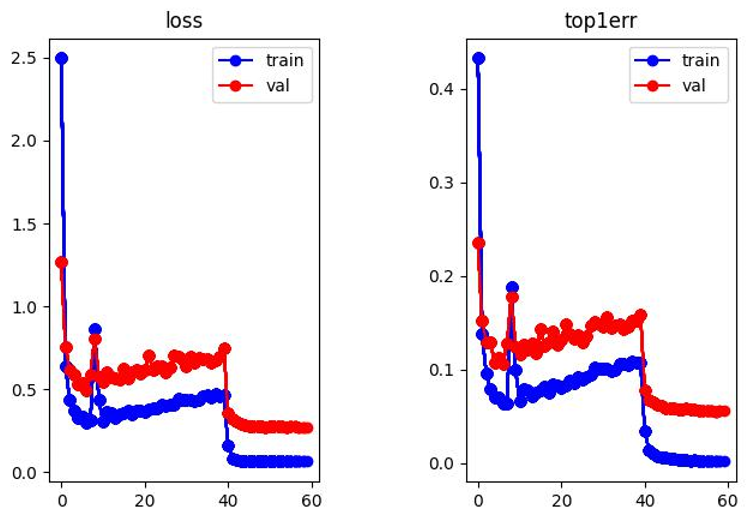
\includegraphics[scale=0.6]{gambar/Train SwinV1_0.png}
  % Keterangan gambar yang diinputkan
  \caption{Grafik Loss dan Top 1 Error dari Swin Transformer V1 Parameter 1 Iterasi 1}
  % Label referensi dari gambar yang diinputkan
  \label{fig:grafiklossdantop1errdariswinv1parameter1iterasi1}
\end{figure}

\begin{figure}[ht]
  \centering
  % Nama dari file gambar yang diinputkan
  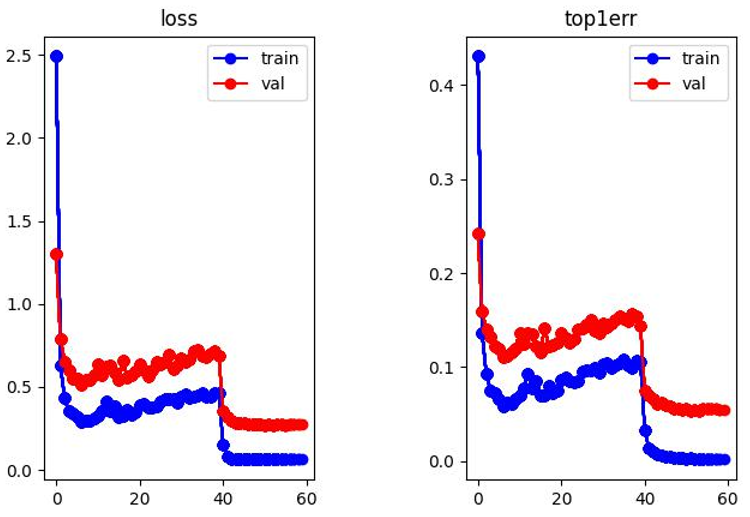
\includegraphics[scale=0.6]{gambar/Train SwinV1_1.png}
  % Keterangan gambar yang diinputkan
  \caption{Grafik Loss dan Top 1 Error dari Swin Transformer V1 Parameter 1 Iterasi 2}
  % Label referensi dari gambar yang diinputkan
  \label{fig:grafiklossdantop1errdariswinv1parameter1iterasi2}
\end{figure}

\begin{figure}[ht]
  \centering
  % Nama dari file gambar yang diinputkan
  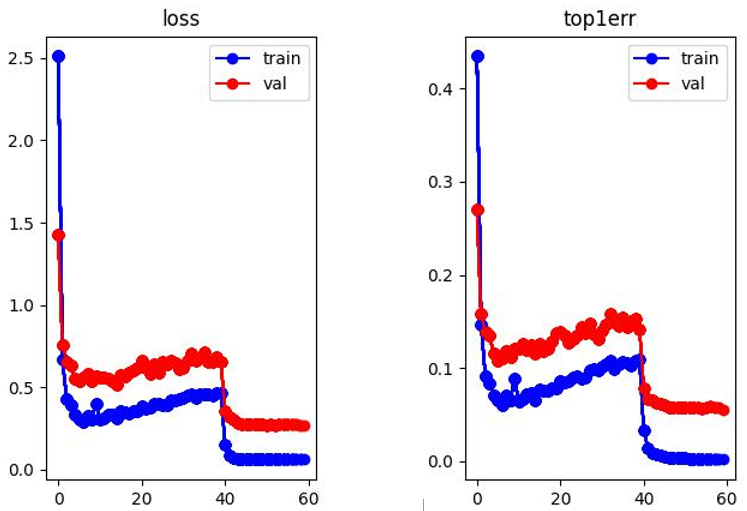
\includegraphics[scale=0.6]{gambar/Train SwinV1_2.png}
  % Keterangan gambar yang diinputkan
  \caption{Grafik Loss dan Top 1 Error dari Swin Transformer V1 Parameter 1 Iterasi 3}
  % Label referensi dari gambar yang diinputkan
  \label{fig:grafiklossdantop1errdariswinv1parameter1iterasi3}
\end{figure}

% Selain gambar grafik diatas, diperoleh pula nilai mAP, rank@1, rank@5, rank@10 dari proses 
% \emph{Testing} pada masing-masing iterasi. Dari tiga kali iterasi tersebut, maka didapatkan 
% rata-rata dari model Swin Transformer V1 Parameter 1. Seluruh nilai iterasi dan rata-ratanya 
% dapat dilihat di tabel 4.1.
Diperoleh pula nilai mAP, rank@1, rank@5, rank@10 dari proses \emph{Testing} pada 
masing-masing iterasi. Seluruh nilai tersebut dapat dilihat di tabel 4.2.

\begin{table}[h!]
  \begin{center}
  \caption{Nilai mAP, Rank@1, Rank@5, dan Rank@10 Swin Transformer V1 Parameter 1}
  \label{tb:NilaimAP,Rank1,Rank5,danRank10ModelSwinTransformerV1Parameter1}
  \begin{tabular}{|l|l|l|l|l|}
      \hline
      \textit{ } & \begin{tabular}[c]{@{}l@{}}\textbf{mAP}\end{tabular} & \begin{tabular}[c]{@{}l@{}}\textbf{Rank@1}\end{tabular} & \begin{tabular}[c]{@{}l@{}}\textbf{Rank@5}\end{tabular} & \begin{tabular}[c]{@{}l@{}}\textbf{Rank@10}\end{tabular}\\ \hline
      \textit{\textbf{Iterasi 1}} & \begin{tabular}[c]{@{}l@{}}0.666313\end{tabular} & \begin{tabular}[c]{@{}l@{}}0.621487\end{tabular} & \begin{tabular}[c]{@{}l@{}}0.818926\end{tabular} & \begin{tabular}[c]{@{}l@{}}0.870864\end{tabular}\\ \hline
      \textit{\textbf{Iterasi 2}} & \begin{tabular}[c]{@{}l@{}}0.667840\end{tabular} & \begin{tabular}[c]{@{}l@{}}0.621487\end{tabular} & \begin{tabular}[c]{@{}l@{}}0.826752\end{tabular} & \begin{tabular}[c]{@{}l@{}}0.869442\end{tabular}\\ \hline
      \textit{\textbf{Iterasi 3}} & \begin{tabular}[c]{@{}l@{}}0.670640\end{tabular} & \begin{tabular}[c]{@{}l@{}}0.624333\end{tabular} & \begin{tabular}[c]{@{}l@{}}0.829242\end{tabular} & \begin{tabular}[c]{@{}l@{}}0.873710\end{tabular}\\ \hline
      \textit{\textbf{Rata-Rata}} & \begin{tabular}[c]{@{}l@{}}0.668264\end{tabular} & \begin{tabular}[c]{@{}l@{}}0.622435\end{tabular} & \begin{tabular}[c]{@{}l@{}}0.824973\end{tabular} & \begin{tabular}[c]{@{}l@{}}0.871339\end{tabular}\\ \hline
  \end{tabular}
  \end{center}
\end{table}

\subsection{Swin Transformer V2 Parameter 1}

Pada Swin Transformer V2 parameter 1, hyper-parameter yang ditentukan yaitu sebagai berikut:

\begin{itemize}[nolistsep]
  \item Epoch = 60
  \item Batch Size = 32
  \item Random Erasing Probability = 0
  \item Learning Rate = 0.05
  \item Warm Epoch = 0
\end{itemize}

\begin{figure}[ht]
  \centering
  % Nama dari file gambar yang diinputkan
  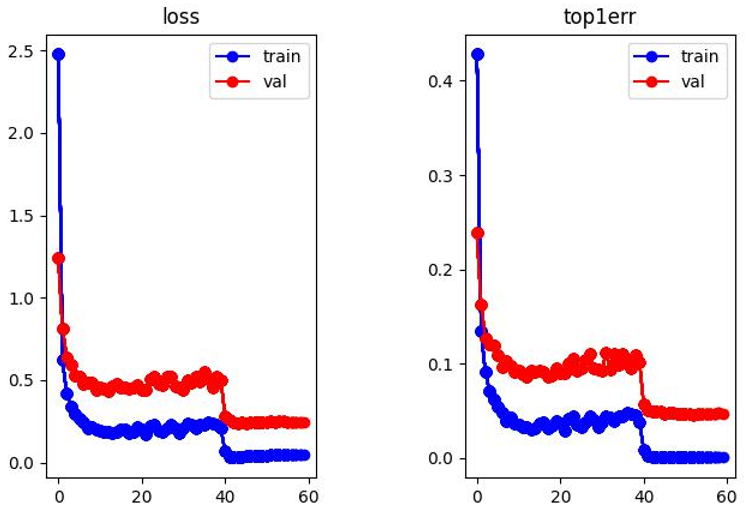
\includegraphics[scale=0.6]{gambar/Train SwinV2_0.png}
  % Keterangan gambar yang diinputkan
  \caption{Grafik Loss dan Top 1 Error dari Swin Transformer V2 Parameter 1 Iterasi 1}
  % Label referensi dari gambar yang diinputkan
  \label{fig:grafiklossdantop1errdariprosestrainingdanvalidationswinv2iterasi1}
\end{figure}

\begin{figure}[ht]
  \centering
  % Nama dari file gambar yang diinputkan
  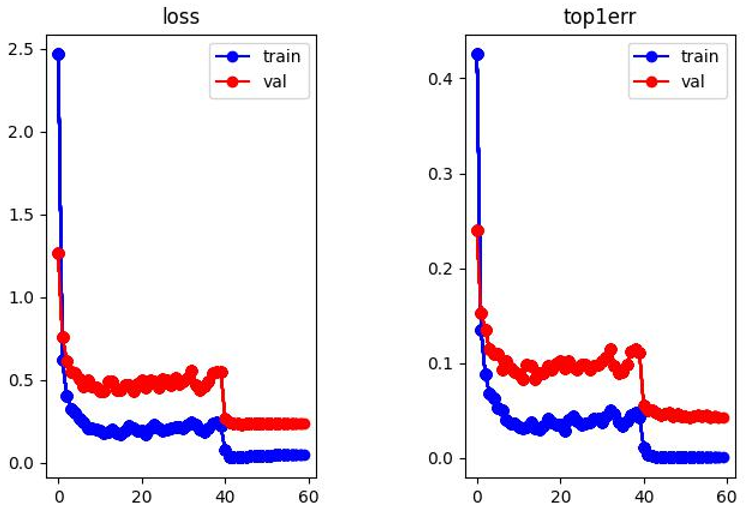
\includegraphics[scale=0.6]{gambar/Train SwinV2_1.png}
  % Keterangan gambar yang diinputkan
  \caption{Grafik Loss dan Top 1 Error dari Swin Transformer V2 Parameter 1 Iterasi 2}
  % Label referensi dari gambar yang diinputkan
  \label{fig:grafiklossdantop1errdariprosestrainingdanvalidationswinv2iterasi2}
\end{figure}

\begin{figure}[ht]
  \centering
  % Nama dari file gambar yang diinputkan
  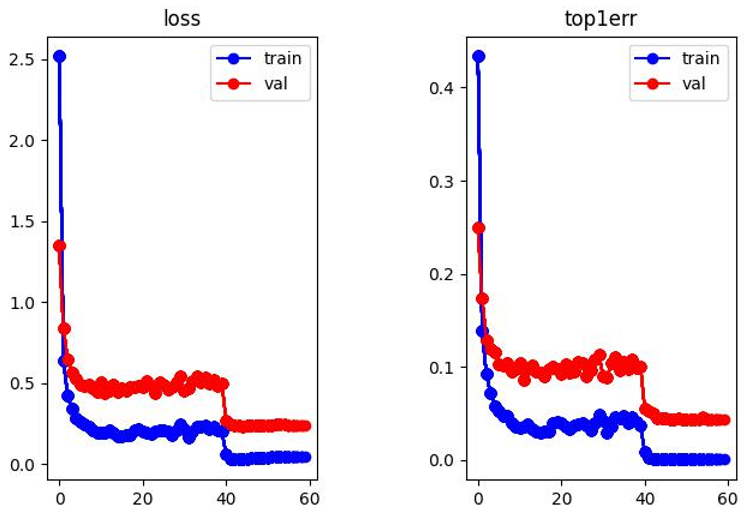
\includegraphics[scale=0.6]{gambar/Train SwinV2_2.png}
  % Keterangan gambar yang diinputkan
  \caption{Grafik Loss dan Top 1 Error dari Swin Transformer V2 Parameter 1 Iterasi 3}
  % Label referensi dari gambar yang diinputkan
  \label{fig:grafiklossdantop1errdariprosestrainingdanvalidationswinv2iterasi3}
\end{figure}

Diperoleh pula nilai mAP, rank@1, rank@5, rank@10 dari proses \emph{Testing} pada 
masing-masing iterasi. Seluruh nilai tersebut dapat dilihat di tabel 4.2.

\begin{table}[h!]
  \begin{center}
  \caption{Nilai mAP, Rank@1, Rank@5, dan Rank@10 Swin Transformer V2 Parameter 1}
  \label{tb:NilaimAP,Rank1,Rank5,danRank10ModelSwinTransformerV1Parameter1}
  \begin{tabular}{|l|l|l|l|l|}
      \hline
      \textit{ } & \begin{tabular}[c]{@{}l@{}}\textbf{mAP}\end{tabular} & \begin{tabular}[c]{@{}l@{}}\textbf{Rank@1}\end{tabular} & \begin{tabular}[c]{@{}l@{}}\textbf{Rank@5}\end{tabular} & \begin{tabular}[c]{@{}l@{}}\textbf{Rank@10}\end{tabular}\\ \hline
      \textit{\textbf{Iterasi 1}} & \begin{tabular}[c]{@{}l@{}}0.666313\end{tabular} & \begin{tabular}[c]{@{}l@{}}0.621487\end{tabular} & \begin{tabular}[c]{@{}l@{}}0.818926\end{tabular} & \begin{tabular}[c]{@{}l@{}}0.870864\end{tabular}\\ \hline
      \textit{\textbf{Iterasi 2}} & \begin{tabular}[c]{@{}l@{}}0.667840\end{tabular} & \begin{tabular}[c]{@{}l@{}}0.621487\end{tabular} & \begin{tabular}[c]{@{}l@{}}0.826752\end{tabular} & \begin{tabular}[c]{@{}l@{}}0.869442\end{tabular}\\ \hline
      \textit{\textbf{Iterasi 3}} & \begin{tabular}[c]{@{}l@{}}0.670640\end{tabular} & \begin{tabular}[c]{@{}l@{}}0.624333\end{tabular} & \begin{tabular}[c]{@{}l@{}}0.829242\end{tabular} & \begin{tabular}[c]{@{}l@{}}0.873710\end{tabular}\\ \hline
      \textit{\textbf{Rata-Rata}} & \begin{tabular}[c]{@{}l@{}}0.668264\end{tabular} & \begin{tabular}[c]{@{}l@{}}0.622435\end{tabular} & \begin{tabular}[c]{@{}l@{}}0.824973\end{tabular} & \begin{tabular}[c]{@{}l@{}}0.871339\end{tabular}\\ \hline
  \end{tabular}
  \end{center}
\end{table}

\subsection{Swin Transformer V1 Parameter 2}
\subsection{Swin Transformer V2 Parameter 2}

% Hasil nilai 
% loss dan top 1 error dari \emph{training} dan \emph{validation} pada setiap model Swin Transformer dapat dilihat pada 
% gambar 4.1 hingga gambar 4.12.

\section{Analisa Hasil}
\label{sec:analisahasil}

% Dari pengujian yang \lipsum[1]

% % Contoh pembuatan tabel
% \begin{longtable}{|c|c|c|}
%   \caption{Hasil Pengukuran Energi dan Kecepatan}
%   \label{tb:EnergiKecepatan}                                   \\
%   \hline
%   \rowcolor[HTML]{C0C0C0}
%   \textbf{Energi} & \textbf{Jarak Tempuh} & \textbf{Kecepatan} \\
%   \hline
%   10 J            & 1000 M                & 200 M/s            \\
%   20 J            & 2000 M                & 400 M/s            \\
%   30 J            & 4000 M                & 800 M/s            \\
%   40 J            & 8000 M                & 1600 M/s           \\
%   \hline
% \end{longtable}

% \lipsum[2-4]
